\subsection{Find the sender of the email}

\begin{frame}{}
\LARGE Naive Bayes Algorithm
\end{frame}


\begin{frame}{Find the sender of the email}
Assume that Ram and Raj exchanged the following emails
\begin{table}
\begin{tabular}{|l|l|}
	\hline
	Ram&Raj\\
	\hline
	I wish you the best&I hope to play tennis tonight\\
	I hope to reach home by 6PM&I hope to win this tournament\\
	I wish to go home early&I hope to buy this car in the next year\\
	I do not want to buy this &I wish to get a good score this time\\
	I hope it rains today&I wish they would come\\
	\hline
\end{tabular}
\end{table}
\vspace{0.3mm}
Who would have sent this email "I wish you would come"
\end{frame}


\begin{frame}{Bag of words - emails }
\begin{figure}
	\centering
	\includegraphics[width=0.8\linewidth]{./Images/BagOfWords}
	\label{fig:bagofwords}
\end{figure}
	Who would have sent this email "I wish you would come"
	\vspace{0.3mm}
	This question can be answered by using Bayes theorem
\end{frame}


\subsection{Bayes Rule}

\begin{frame}{Bayes Theorem}

Let us consider two random variables $X \, and \, Y$. Then
\vspace{0.3mm} Joint probability, $P(X=x,Y=y)$, refers to the probability that the variable $X$ takes the value $x$ and the variable $Y$ takes the value $y$.
\vspace{0.3mm}
The conditional probability $P(Y=y|X=x)$ refers to the probability that the variable $Y$ takes the value $y$ given the observation the variable $X$ takes the value $x$
\begin{align}
P(X,Y) &= P(Y|X)\times P(X) = P(X|Y)\times P(Y)\\
P(Y|X) &= \dfrac{P(X|Y)P(Y)}{P(X)}
\end{align}
\end{frame}

\begin{frame}{Mapping Bayes theorem to email classification problem}
\begin{itemize}
\item Map Bayes theorem using the statistical properties of the data
\item Let $\textbf{X} = $ and $Y$ represent the random variables, where $\textbf{X}$ is a set of attributes or is a attribute variable and $Y$ represent a class.
\item The relationship between $\textbf{X}$ and $Y$ can be found using the conditional probability  $P(Y|\textbf{X})$
\item The conditional probability $P(Y|\textbf{X})$ is known as posterior probability of Y
\item $P(Y)$ is known as the prior probability
\item In the classification problem, it is important to learn the parameters $P(Y|\textbf{X})$. Given the attributes of the email (TF,TF-IDF), find the class to which the email belongs - in this case the person who sent it.
\end{itemize}

\vspace{0.5 ex}
The parameters are obtained from the training data - the corpus of emails written by Ram and Raj. During the training process, we will learn $P(Y|\textbf{X})$ for every word in the corpus
\end{frame}


\begin{frame}{Supervised Classification}
\begin{itemize}
	\item Set of input parameters/attributes $\textbf{X} = {X_1,X_2,\ldots, X_m}$and a fixed set of classes $Y = {y_1,y_2,\ldots, y_n}$
	\item Every element of the training set, $D={d_1,d_2,\ldots,d_n} $ is manually assigned a class
	\begin{itemize}
		\item [] $(d_1,y_1), (d_2,y_2),(d_3,y_1), \ldots$
	\end{itemize}
	\item Goal is to learn the classifier, so that it can map a new document $\hat{d}$ to any of the classes, $y \in Y$
	\item Bayes classifier would assign a probability based on the observation to the new document to aid the class selection
	\item The probability score for each class is computed as given by the equation $P(Y|\textbf{X}) = \dfrac{P(\textbf{X}|Y)P(Y)}{P(\textbf{X})}$
	\item The class will be found using $\displaystyle \argmax_{y\in Y} P(Y|\textbf{X})$
\end{itemize}
\end{frame}

\begin{frame}{Estimating the conditional Probability $P(X_i|Y)$}
\begin{align}
\hat{y} &=\argmax_{y\in Y} P(Y|\textbf{X})\\
&=\argmax_{y\in Y}P(\textbf{X}|y)P(y)\\
&=\argmax_{y\in Y}P(y)P(X_1,X_2,X_m|Y)\\
&=\argmax_{y\in Y}P(y)P(X_1|y)\times P(X_2|y)\times \ldots P(X_m|y)\\
&=\argmax_{y\in Y}P(y)\prod_{i=1}^{m}P(X_i|y)
\end{align}
\end{frame}

\begin{frame}[shrink]{Training}
\begin{multicols}{2}
\begin{enumerate}
	\item Prior probability -
	$P(y) = \dfrac{Count(y)}{Count(Y)}$
	\item Learn $P(X_1|y) = \dfrac{Count(X_1,y)}{Count(Y)}$
\end{enumerate}
\begin{table}
	\begin{tabular}{|p{3cm}|p{3cm}|}
		\hline
		Word&Frequency\\
		\hline
		&\\
		&\\
		&\\
		&\\
		&\\
		&\\
		&\\
		&\\
		&\\
		&\\
		&\\
		&\\
		&\\
		\hline
	\end{tabular}
\end{table}
\end{multicols}

\end{frame}
%\begin{frame}[shrink=10]{Naive Bayes Rule for Document Classification}
%\begin{itemize}
%	\item Bayes' rule describes the probability of an event, based on prior knowledge of related conditions.
%	\item Naive Bayes is a simple yet a powerful tool for classification/prediction.
%	\item Uses historical information to find the best hypothesis
%	\item Relies on the \textbf{\textit{Bag of Words } }
%	\item Does not depend on the position of the word in the document
%	\item Likelihood estimate uses the frequency of the word in the given document
%\end{itemize}
%\begin{align*}
%\textit{Bayes Rule - } \ P(c|d) &= \frac{P(d|c)P(c)}{P(d)}= \frac{\text{Count of }(d,c)}{\displaystyle \sum_{w \in V}(w,d)}
%\end{align*}
%
%\begin{multicols}{2}
%	where\\ $P(c|d)$ is \textit{Posterior probability},\\
%	$P(d|c)$ is the \textit{likelihood},\\
%	$P(c)$  \textit{class prior probability} and\\
%	$P(d)$ is the \textit{predictor probability}
%	\columnbreak \vfill
%	A \textit{prior probability} is a value originally obtained before any additional information is obtained.
%	A \textit{posterior probability} is a value that is revised by incorporating additional information that is obtained at a later point in time.
%\end{multicols}
%\end{frame}

%\begin{frame}
%Find the sender using the historical information given in the table
%\begin{multicols}{2}
%\begin{center} {\textbf{Historical Information}}
%	\begin{tabular}{||c|c||}
%		\hline
%		Ram & Raj\\
%		\hline
%		Hope(0.8) &Hope(0.5)\\
%		\hline
%		Play (0.1)& Play(0.4)\\
%		\hline
%		Energy(0.1)& Energy(0.1)\\
%		\hline
%	\end{tabular}
%\end{center}
%\columnbreak \vfill
%\noindent
%\textbf{Priors}:\\
%P(Ram) = 0.5 \text{ and } \\
%P(Raj) = 0.5\\
%\end{multicols}
%\begin{align*}
%&P(Ram|Play,Hope) = \frac{P(Play,Hope|Ram)*P(Ram)}{\sum P(Play,Hope)} = 0.04\\
%&P(Raj|Play,Hope) = \frac{P(Play,Hope|Raj)*P(Raj)}{\sum P(Play,Hope)} = 0.10	\\
%&	\text{Ram:} = 0.04/\left(0.04+0.1 \right) = 0.29
%\text{ and Raj:} 0.01/0.14 = 0.71\\
%\end{align*}
%\end{frame}

	\subsection{Hand on Exercise 1 }
	\begin{frame}{Hands on Exercise 1 - Find the sender of the email}
		Assume that Ram and Raj share emails exchanged emails using the words given in the table. A new email arrives with just three words -
		\textbf{\textit{motivate, profit and product}}.
		Find the sender using the historical information given in the table\\
		\begin{center}
			Historical Information\\
			\medskip
			\begin{tabular}{||c|c||}
				\hline
				Ram &Raj\\
				\hline
				motivate(0.24) & 		motivate(0.05)\\
				\hline
				profit(0.3)& 			profit(0.35)\\
				\hline
				product(0.26)& 			product(0.35)	\\
				\hline
				leadership(0.08)&		leadership(0.15)\\
				\hline
				operations(0.12) &		operations(0.10)\\
				\hline
			\end{tabular}
		\end{center}

	Who would have used these words (motivate, profit and product) in the email ?
	\\
		Is it possible to apply this technique to identify the sentiments of a movie review with two classes \textbf{Good} and \textbf{bad}?
	\end{frame}
	\subsection{Hands on Exercise 2}
	\begin{frame}{Hands on Exercise 2 - Product Sentiments}
		Assume the following likelihoods for each word being part of a positive or
		negative review, and equal prior probabilities for each class - positive and negative ($P(positive)=0.5 \text{ and } P(negative) = 0.5$)
		\begin{center}
		\begin{tabular}{||c|c|c||}
			\hline
			word&positive&negative\\
			\hline
			I&0.09&0.16\\
			\hline
			love &0.07& 0.06\\
			\hline
			to&0.05&0.07\\
			\hline
			fill& 0.29&0.06\\
			\hline
			 credit& 0.04&0.15\\
			 \hline
			 card& 0.08&0.11\\
			 \hline
			 application&0.06&0.04\\
			 \hline
		\end{tabular}
	\end{center}
		What class Naive Bayes classifier would assign to the sentence {\small "I do not like to fill in the application form?"}
	\end{frame}